\documentclass{article}

% 8 pages MAX!

% if you need to pass options to natbib, use, e.g.:
% \PassOptionsToPackage{numbers, compress}{natbib}
% before loading nips_2016
%
% to avoid loading the natbib package, add option nonatbib:
% \usepackage[nonatbib]{nips_2016}

\usepackage{nips_2018}

% to compile a camera-ready version, add the [final] option, e.g.:
% \usepackage[final]{nips_2016}

\usepackage[utf8]{inputenc} % allow utf-8 input
\usepackage[T1]{fontenc}    % use 8-bit T1 fonts
\usepackage{hyperref}       % hyperlinks
\usepackage{url}            % simple URL typesetting
\usepackage{booktabs}       % professional-quality tables
\usepackage{amsfonts}       % blackboard math symbols
\usepackage{nicefrac}       % compact symbols for 1/2, etc.
\usepackage{microtype}      % microtypography
\usepackage{graphicx}

\title{Feedforward error propagation in a deep closed loop neural network}

% The \author macro works with any number of authors. There are two
% commands used to separate the names and addresses of multiple
% authors: \And and \AND.
%
% Using \And between authors leaves it to LaTeX to determine where to
% break the lines. Using \AND forces a line break at that point. So,
% if LaTeX puts 3 of 4 authors names on the first line, and the last
% on the second line, try using \AND instead of \And before the third
% author name.

\author{
  Bernd Porr\\
  Glasgow Neuro LTD\\
  United Kingdom\\
  \texttt{bernd@glasgowneuro.tech} \\
  %% examples of more authors
  %% \And
  Paul Miller \\
  Glasgow Neuro LTD \\
  United Kingdom \\
  \texttt{paul@glasgowneuro.tech}
}

\begin{document}

\maketitle

\begin{abstract}
  Recent advances in neurophysiology suggest that a neural network can transmit two separate signals with distinct functions, via cross-frequency
  coupling. We propose that one signal carries
  behaviourally relevant activity and the other an error signal
  controlling plasticity, and this allows error-based learning in such a
  deep network. We have embedded this network in a closed loop
  scenario, where an error signal is propagated \textsl{forwards} from its input via its
  deeper layers to its output, with the goal of minimising the error
  signal. We demonstrate its performance with a 1st person shooter
  game.
\end{abstract}

\section{Introduction}
There is strong neurophysiological evidence that different brain
oscillations enable the brain to carry separate information via the
same synapses and neurons in a forward fashion
\cite{Canolty2010}. These streams, represented by different
frequency bands, control plasticity in specific ways, with the higher
frequency components affecting plasticity \cite{Bliss73},
and the lower ones being relevant for behaviour \cite{Luescher2012} while keeping plasticity constant. This means that error signals are
propagated in a forward fashion from the inputs of the network to its
outputs, altering plasticity while progressing through the network.

On a system level, brain decision networks receive an error signal in
the striatum in the form of dopaminergic innervation \cite{Schultz97}, but
their cortical targets receive very little dopamine
\cite{Groenewegen1993}. This poses a problem of how higher level
decision-making receives errors whilst also showing more flexibility than rigidly aiming for a reward. A single
reward prediction error cannot account for the large behavioural
flexibility that higher animals and humans show.

Propagating errors from the input to the output is the realm of
reinforcement learning, in which actions feed back from the environment
and then are evaluated with the help of sensor
inputs\cite{Verschure91,Dayan1992,Sutton88,Sutton98,PorrNecoInvco2003,Woergoetter2005}. In
the simplest case an error signal can be achieved by a reflex
\cite{Verschure91,PorrNecoInvco2003}, where the agent reacts to
unexpected changes in their environment. In the language of control
\cite{Phillips2000} this means that a desired state should be
maintained as closely as possible. The difference between the desired
state and the actual state is the error signal of the control loop, and
can be used not only to trigger a behavioural action but also fed
into a neural network. We demonstrate this in our novel
architecture.

In this paper we present a novel deep network algorithm for closed
loop systems called ``Deep Feedback Learning'' (DFL) -- this propagates an error signal in a forward fashion through its network. The input is directly driven by the error signal, but the deeper
layers receive weighted sums of the error from the previous layers.
We demonstrate this in a 1st-person shooter game using Vizdoom.

\begin{figure}[!ht]
  \centering
  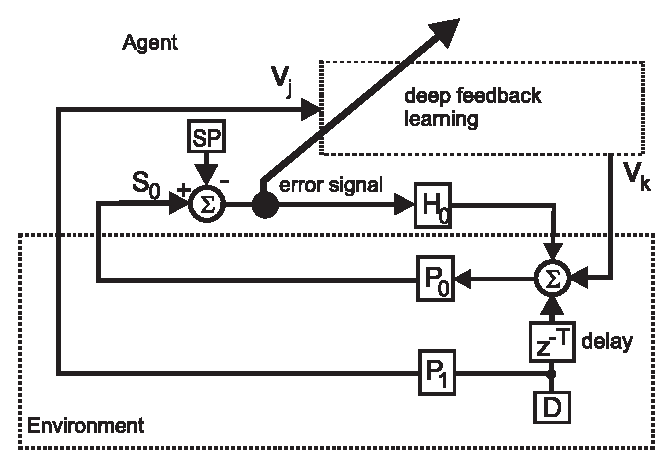
\includegraphics[width=0.75\columnwidth]{closed_loop}
  \caption{A closed loop system with a setpoint $SP$, transfer function $H_0$ and the
    environment $P_0$ which needs to work against unpredictable disturbances $D$.
    The error signal tunes a deep neuronal network, which has inputs
    $V_i$ that predict the disturbances. The network tries to pre-empt these
    disturbances and generate an appropriate action $V_k$. The transfer
    functions here are indicated with capital letters and are in the
    sampled z-domain.
    \label{closed_loop}}
\end{figure}

\section{Closed loop learning}
Before we describe the algorithm, we need to place it in a closed loop
context. Fig.~\ref{closed_loop} shows the entire closed loop system,
with the deep feedback learning as a black box for now. The idea is
that we have a fixed closed loop which is able to fend off
disturbances, such as an unexpected bend on a road or the sudden
appearance of an enemy. This fixed loop then takes appropriate action
to solve this disturbance, e.g. correcting a car's steering, targeting
food or aiming towards and shooting an enemy. In formal terms we have
a setpoint $SP$ which compares the input of organism to a desired
input. If the input deviates from the setpoint an action is generated
with the transfer function $H_0$. This action then eliminates the
disturbance $D$ and arrives via the environmental transfer function
$P_0$ at the input again; thus, the loop is closed. However, we are
not so much interested in the design of the closed loop but rather
that it generates an \textsl{error signal}. The error signal is
non-zero if a disturbance has happened, and this can be used to tune our
deep feedback learning network.

Our network receives additional inputs which are able to predict the
disturbance, and thus prevent the trigger of the feedback loop. These
additional inputs are provided via $V_i$ where we have shown one
pathway and possible additional inputs as a dashed line in
Fig~.\ref{closed_loop}).
For example a video camera or eyes can provide images of the way ahead,
or of an enemy prior to attacking. Our algorithm has the task of using the error
signal to tune its network and to minimise this error, as described next.

\begin{figure}[!ht]
  \centering
  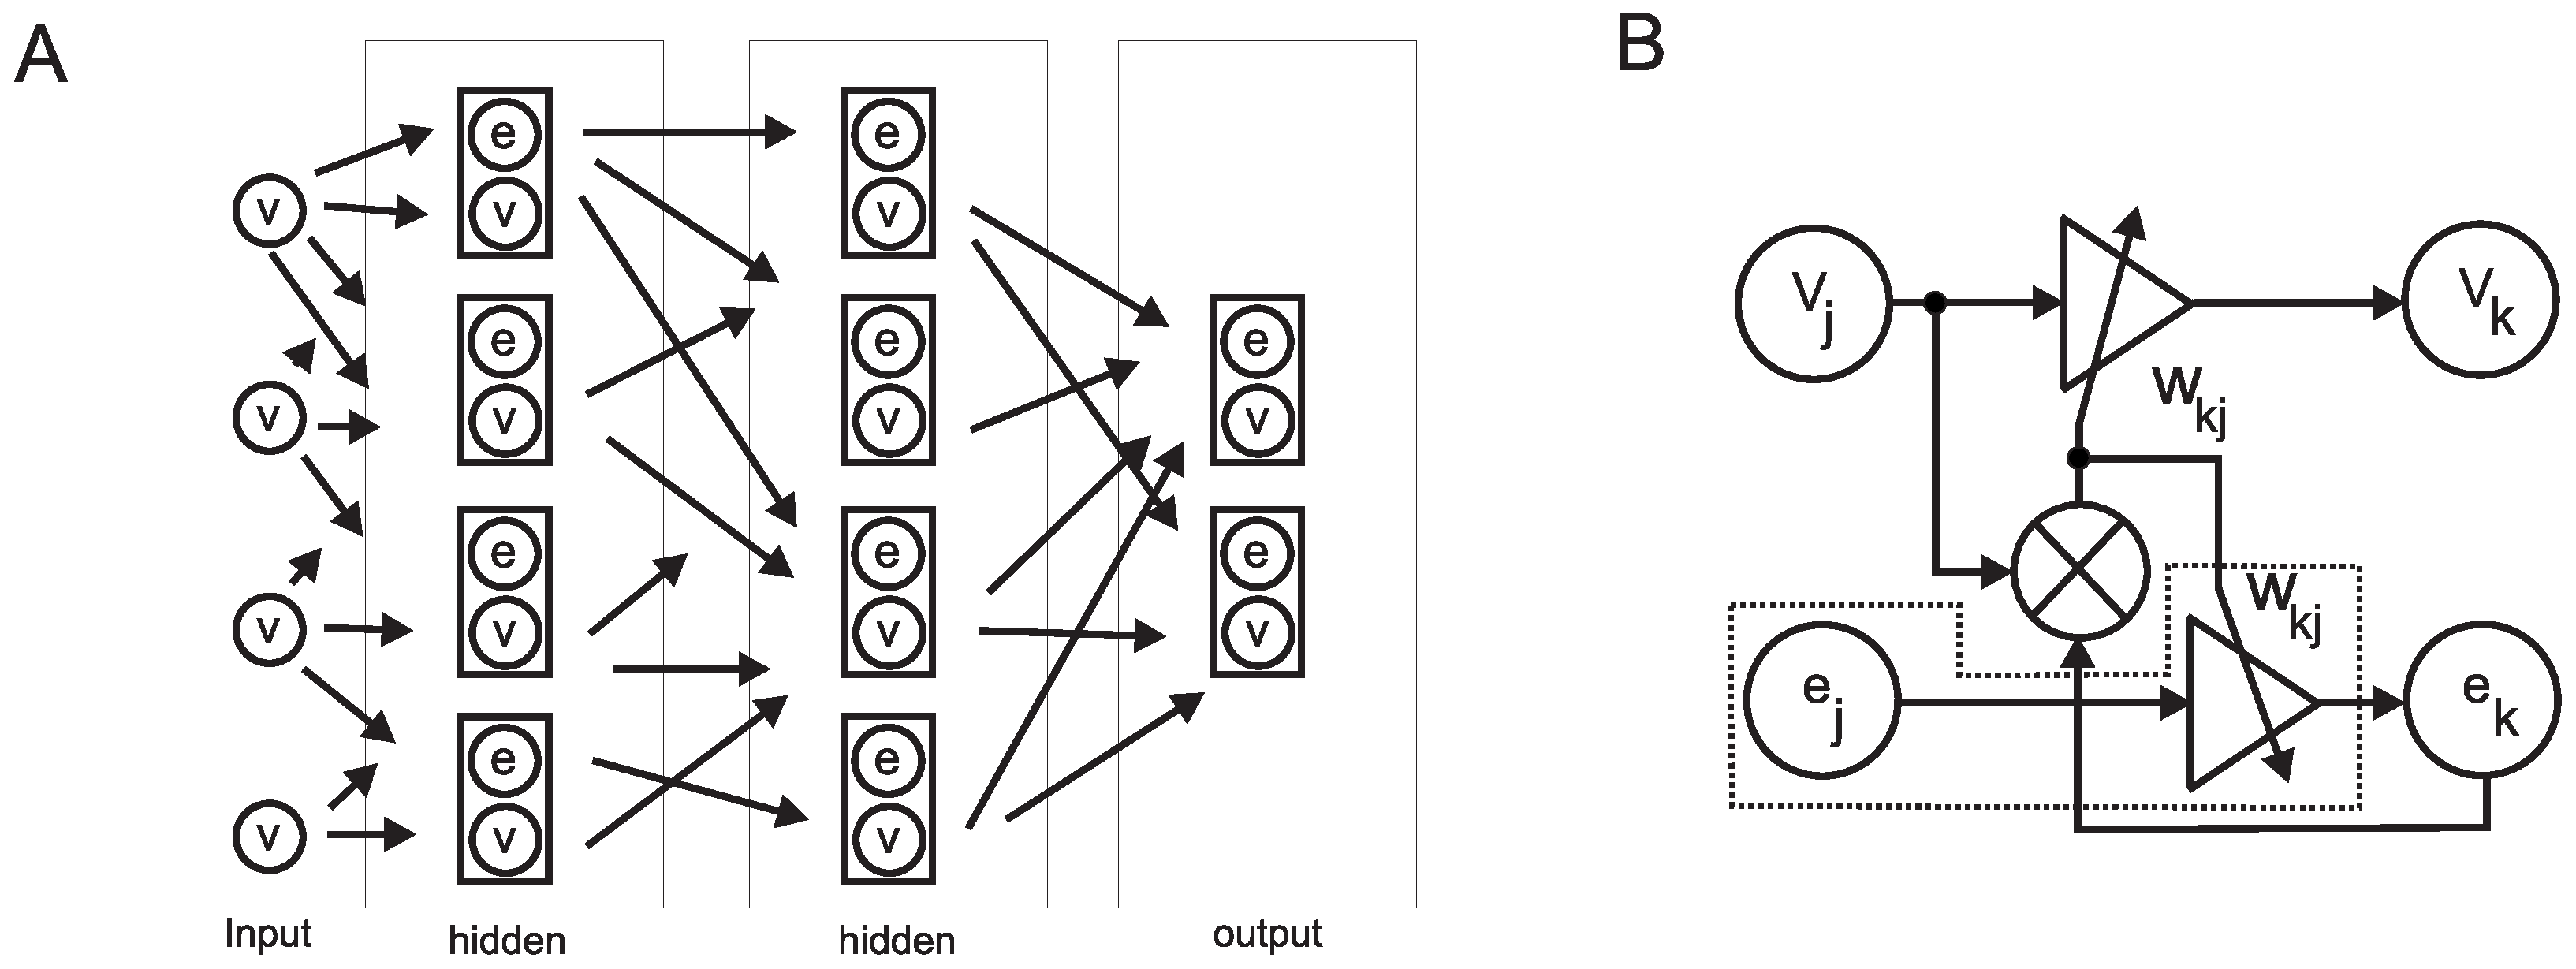
\includegraphics[width=\columnwidth]{netw_together}
  \caption{A) Network overview. With the exception of the input layer, every
    neuron is a composite cell with an activation $v$ and an error
    term $e$. These are propagated through the network in a weighted
    fashion in parallel.  B) Computation in a single composite cell.
    The presynaptic activities $v_j$ and error signals $e_j$ are used
    to perform correlation based learning and change the weight
    $w_{jk}$ which weights for both activity and error propagation into the next
    layer. The contents of the dotted box only exist for the deeper
    layers as also illustrated on the left with the input layer
    having only activities $v$, but no errors. \label{netw_together}}
\end{figure}


\section{Deep feedback learning}
We define a network with an input layer, hidden units and an output
layer which can all have different numbers of neurons (see
Fig~\ref{netw_together}A). In contrast to traditional
networks, every layer (except for the input layer) consists of two
summation nodes: the actual activity and an error signal. These
are processed in two parallel streams.

Let us first focus on the network activity. We define a multi-layered
network, where every neuron in any layer is a standard computational unit that
calculates a weighted sum $v_k$ of its inputs $v_j$ and then applies
an activation function $\Theta(x) = \tanh(x)$:
\begin{equation}
  v_k = \Theta\left( \sum_j w_{jk} v_{j} \right) \label{act_sum}
\end{equation}
The activity flows from neurons in layer $v_j$ to neurons in
layer $v_k$ multiplied by the weights $w_{jk}$, and this
is then repeated in the next layer. For a network with
$N$ layers we have then $N-1$ sets of weights $w_{jk}$. Note that these
indices are just examples and we start with $i$ for the 1st layer and then
$j$ and so on.

The weight changes are then updated in a semi-Hebbian fashion:
\begin{equation}
  w_{jk}(t+1) = w_{jk}(t) + \gamma v_j(t)  e_k(t) + \mu \Delta w_{jk}(t) \label{learningRule}
\end{equation}
where $v_j(t)$ is the presynaptic activity and $e_k(t)$ is an error
signal attached to the postsynaptic neuron, so the correlation is
calculated between input signals and the error signal, with the
standard parameters learning rate $\gamma$ and momentum $\mu$.

We now describe the error signal propagation. As outlined above, the
error signal emerges from the feedback loop, and is injected into the
network at the 1st hidden layer as the ``postsynaptic'' activity. The
weight change for this 1st layer can then be calculated directly with
Eq.~\ref{learningRule} by setting $e_k$ to the error signal of the
feedback loop (see Fig.~\ref{closed_loop}).

For the deeper layers, the error signal is computed as a weighted
sum of the error signals from the previous layer:
\begin{equation}
  e_k = \frac{\left( \sum_j w_{jk} e_{j} \right) \Theta^\prime (v_k) }{\frac{\sum_j {|w_{jk}|}}{\sum_j 1}}
  \label{deepError}
\end{equation}
where the $\Theta^\prime (v) = 1 - v^2$ is the derivative of the
activation function $\Theta(v)$: this limits learning when the unit
approaches saturation, as in backprop. The norm guarantees that
the error propagates through all layers and does not vanish from
layer to layer due to small weights.

A simplified data flow diagram of the learning performed in each layer
is shown in Fig~\ref{netw_together}B, where we see the two processing
streams: both the activity $v_j$ and error signal $e_j$ are weighted
by $w_{jk}$, and summed separately in the next layer. Remember that
for the 1st hidden layer, the error is just the error signal
directly injected from the feedback loop. The diagram omits the error
normalisation, scaling and activation derivative in order to focus on
the main point that learning happens between the error signal and the
presynaptic activity.

Learning is therefore performed in three steps: first the activity is
propagated through the network, then the error signal is propagated
via the \textsl{same} weights, and finally the weights are adjusted. Thus,
both the error signal and the activity are propagated in a forward
fashion. Learning itself can be interpreted as \textsl{heterosynaptic} for the
activity $v_j$ and \textsl{Hebbian} for the error $e_j$.


\section{Derivation of the learning rule}
We start from the assumption that a single neuron using heterosynaptic
plasticity is able to eliminate an error signal
\cite{Porr2006ICO}. Because of the exploding complexity of closed loop
learning we focus here how an error signal $X_0$ should be propagated
to deeper layers from its input by using the approach in
\cite{Mehta1986}, taking partial derivatives in the z-space and assuming
that weight development in time is slow in comparison to the closed loop
dynamics.  Let us assume two layers $j$ and $k$ where the input signals
to the deep network are signals with index i so that we have $V_i,
V_j$ and $V_k$. The error signal, $X_0$ (see Fig.~\ref{closed_loop}), can be expressed as
\begin{equation}
  X_0 = \frac{P_0 \left[ V_k V_J + D z^{-1} \right]}{1-P_0 \rho H_0}
\end{equation}
We know that a weight change $\Delta w$ calculated by correlating $X_0$ with an input
$V_i$ leads to convergence in a closed loop system. This can be expressed
as:
\begin{equation}
  \Delta w_{ij} = X_0(z) V_i(-z)
\end{equation}
We now need to show that if we have deeper weights such as $w_{jk}$
that these will change in the same way as those of the input layer. In
order to establish this, we look at small weight changes in $w_{jk}$ and relate them to the input weights $w_{ij}$.
\begin{equation}
    \frac{\partial X_0}{\partial w_{jk}} =
    \frac{\partial X_0}{\partial V_j}
    \frac{\partial V_j}{\partial V_k}
    \frac{\partial V_k}{\partial w_{jk}}
\end{equation}    
where
\begin{equation}
\frac{\partial X_0}{\partial V_j} = \frac{P_0 V_k}{1-P_0 \rho H_0}
\end{equation}
If we assume for now that the layers consist only of linear neurons:
\begin{eqnarray}
  V_k &=& \sum_j w_{jk} V_j \\
  V_j &=& \sum_i w_{ij} V_i
\end{eqnarray}
then this yields:
\begin{eqnarray}
    \frac{\partial X_0}{\partial w_{jk}} &=&
    \frac{P_0 V_k}{1-P_0 \rho H_0}
    \frac{\partial V_j}{\partial V_k}
    V_j \\
                                        &=&
    \frac{P_0 V_k}{1-P_0 \rho H_0}
    \frac{\partial V_j}{\partial V_k}
    \sum_i w_{ij} V_i
\end{eqnarray}    
  We can now multiply this equation with $V_i(-z)=V_j^-$ to indicate a correlation, yielding:
\begin{equation}
    \frac{\partial X_0}{\partial w_{jk}} V_i^- =   
    \frac{P_0 V_k}{1-P_0 \rho H_0}
    \frac{\partial V_j}{\partial V_k}
    \underbrace{\left( \sum_{i^\prime} w_{i^\prime j} V_{i^\prime} \right)}_\textrm{\tiny deep layer error signal} V_i^-
\end{equation}
This means that if we introduce a small change in the deeper weights $w_{jk}$
they will depend on the weighted covariance at the input where this correlation
at the input propagates, weighted by the input weights $w_{ij}$, to the deeper layer
$w_{jk}$. This shows that the error signal is propagated in a weighted
fashion to deeper layers. Note that this is not a stability proof but rather
the derivation of the network structure, using a similar trick to deep learning
but in closed loop and forward fashion. For a stability analysis one needs
to take into account for the non-linear activation functions and unroll the
partial derivative $\frac{\partial V_j}{\partial V_k}$, whose derviative depends
again on the entire closed loop. However, this is not of practical relevance
because the environmental transfer function is rarely known.
    
\section{Shooter game}
In this scenario, we try to learn to play a first-person shooter
purely from visual inputs. We use the Vizdoom
(http://vizdoom.cs.put.edu.pl/) environment for this purpose, and
train a controller to play against a single pretrained bot from Intel
that ran in the Vizdoom 2016 competition. The setup was as follows:

The images returned from Vizdoom are RGB 160x120. We rendered the
enemy in blue, and formed a reflex signal by finding the bounding box
of the pixels closest to that colour. Note that the reflex is slow and
also inherently noisy, as other events in the game are also rendered
blue (e.g. the ‘flashes’ that happen at respawns). The reflex also
fails at times when the enemy is too distant or too close to the
camera. For learning, we only supply the network with the greyscale
image (Fig.~\ref{shooter_results}G) flattened into a vector of $19200$
inputs, so it is forced to discover purely spatial cues. The reflex is
computed relative to the image centre, so a negative value implies the
enemy is on the left. Shooting behaviour is entirely hardwired: if an
enemy is detected within a threshold of the image centre, the bot
fires. Note that the bot's only actions are to rotate in the plane,
and shoot -- it does not translate (but the enemy does). Instead of
separate outputs for left and right, we have a single value produced
by 3 neurons acting at different sensitivities:
\begin{equation}
\Delta \theta = g_{err}\, \mathrm{error} + g_{net} \left( 10 v_0 + 3 v_1 + v_2 \right)
\end{equation}
where $v_0, \ldots, v_2$ are the network outputs, and $\Delta \theta$
is the change in orientation.


\begin{figure*}[!ht]
	\centering 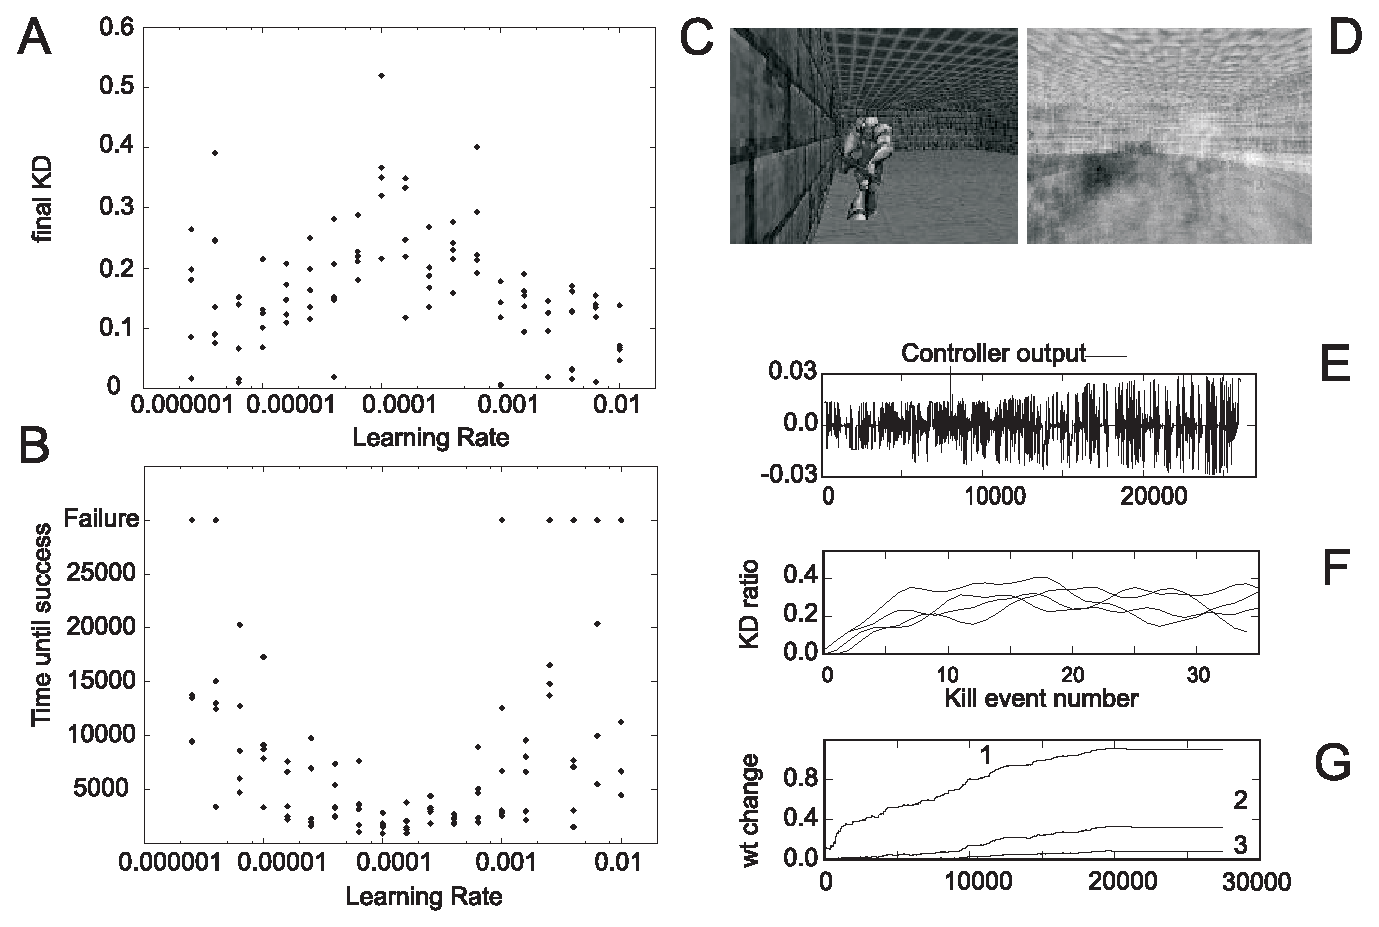
\includegraphics[width=\textwidth]{FPSFig7}
	\caption{A) KD at end of trial. B) Time to success vs learning
          rate - success is if the smoothed KD ratio reaches a
          threshold of 0.15. C) $\Delta \theta$, the rate of change in
          bot's orientation against simulation step number, purely
          from the DFL output, in arbitrary units. D) KD learning
          curves - the time series of kills/deaths is filtered with a
          2nd order lowpass filter to get a moving average, plotted
          against kill event number. E) Euclidean distance of weights
          for each layer from their initial point, against learning
          step. F) Example input weights. G) Example input frame.
          Parameters: 19200 inputs from grayscale image; 2
          hidden layers of 5 units each; no filterbank. Inputs were
          normalised to zero-mean, unit variance. Learning rate in D
          and E was 0.0001.
		\label{shooter_results}}
\end{figure*}

\subsection{Results}
As before, we see that the controller outputs steadily increase over
time (Fig.~\ref{shooter_results}C). With a high value of $g_{net}$,
the bot can make very rapid aiming movements. This has the advantage
that the error can in principle be reduced very quickly; it also
causes the bot to sometimes make large rotations even when the enemy
is out of the field of view, which helps with exploration. On the
other hand, it can cause the aiming to overshoot and oscillate around
the target.  The weights grow in a similar pattern to before, although
their progression is less smooth, due to the more discontinuous nature
of the error signal (Fig.~\ref{shooter_results}E). The different
scales are likely due to the inputs having more dimensions.

Unlike the Line Follower, it is not possible here to drive the error
to zero, as there are discontinuities when either bot respawns, and so
the enemy will often abruptly appear somewhere in the image. One
performance measure is simply how often our bot is killed vs how often
it kills the enemy. In gaming, this is called the kill/death ratio,
and we plot some smoothed KD curves in Fig.~\ref{shooter_results}D. To
do statistics, we measure the time taken to reach a threshold KD of 0.15 -
Fig.~\ref{shooter_results}B shows this as a function of learning
rate. As before, there is a stable region in the middle where learning
is consistently successful. We also plot the smoothed KD for the final
step of each trial(Fig.~\ref{shooter_results}A); although a noisy
measure, the same pattern emerges. Over time, the input weights blur
the background, leaving dark and light blobs to detect the enemy and
generate an aiming response (Fig.~\ref{shooter_results}F).

Note that this is only one skill of a functioning FPS bot, as a real bot would
require additional skills such as seeking rewards (e.g. finding health packs) and
navigating the environment (e.g. avoiding collisions). Future research
will investigate whether the DFL approach can be used to acquire such
skills, using the same fundamental approach of learning to anticipate
a prewired behaviour.


\section{Discussion}
We have shown that a deep network which propagates its errors in a
forward fashion from its inputs to its outputs is able to solve closed
loop learning tasks. We have demonstrated this in a first person
shooter game.

Plasticity has always been hotly debated in neurophysiology -- the
general understanding is that a large postsynaptic Calcium
concentration causes LTP \cite{Malenka99,Bennett2000} and a low one
causes LTD \cite{Mulkey1992}. This requires a strong presynaptic
drive to achieve a strong postsynaptic activity, and with that Ca
influx \cite{Meunier2017}. In mathematical terms this would just lead
to self-amplification of the synaptic weight, where strong presynaptic
activity would causes greater postsynaptic activity and in turn stronger
weights, and so on. However, suppose the learning signal and the
actual activity were transmitted via the same synapse but were
fundamentally separated \cite{Lindsay2017}, for example by using
different frequencies: high frequency potentials could cause
plasticity changes while low frequency potentials propagate
behaviourally-relevant activity \cite{Canolty2010}. DFL can provide
here a mechanism that allows stable behaviourally-relevant learning
driven by heterosynaptic plasticity and Hebbian learning for the error
signal, with the stability arising from the fact that it is constantly
corrected by the error signal.

Looking at a system-wide perspective, one can see DFL as a flexible
actor which has a high degree of freedom in generating actions, as long as they
minimise the error. For example in the basal ganglia the striatum is
seen as an actor receiving an error signal via dopamine, the famous
reward prediction error \cite{Schultz97} which is understood as being
closely related to the error of temporal difference learning
\cite{gurney98:_basal_gangl_action_selec_devic}. It is curious that
the striatum receives the error signal but both downstream neurons in
the basal ganglia and upstream in the cortex receive little
dopaminergic modulation \cite{Beckstead1979}. However, plasticity is
not just limited to the striatum, but happens in all brain areas, so
it makes sense to propagate this error signal further back into the cortex
\cite{Groenewegen1993} where high level decision-making takes place.
In the language of TD learning \cite{Sutton87} this means that we
have a distributed actor where the first layer is modulated by
reward prediction error, and then the following stages, that project
back to the cortex, use instead cross frequency coupling
as described above \cite{Lipski2017}.

Given that the error is propagated from the input to the
output, the novel aspect here is that the more layers DFL has, the more remote it
is from the immediate error feedback. This allows for
increased flexibility which is then a function of the number of layers, and
creates an actor which is far less rigid than a standard Q-learner
\cite{Dayan1992}. The actions can be substantially varied as
long as the error signal can eventually be minimised, and the variability will be
more pronounced with more hidden layers. In other words, the more
hidden layers we have, the more behavioural flexibility the agent will
show. In a biological context this means that as cortical processing
takes over in the deeper stages, it also can develop more flexibility
while still receiving \textsl{distributed} error signals rather than 
a global one.

A different stance about synaptic plasticity (and ultimately how
autonomous agents learn) has been taken by the deep learning
community, which has recently claimed that error backpropagation is
biologically realistic \cite{Lillicrap2016,Roelfsema2018}. This has
been demonstrated in a network with one hidden layer by introducing a
separate feedback pathway from the output of the network to this
hidden layer, but this does not take account the cortico-striatal network mentioned above. While this shows promising results for
abstract models of biologically inspired decision making, the underlying
backprop operates in an open loop fashion (i.e. output control), and thus
contradicts the requirement for an agent to control its inputs.

\cite{Guo2014} takes a different direction, and present an
approach that uses backprop to solve closed loop problems. To turn the
open loop backprop into a closed loop algorithm, they embedd it into
Q-learning which is itself closed loop. However, even given its major
performance advances, the main drawback is the
discrete state space, which makes it hard to solve analogue problems,
and Q-learning is not biologically realistic when compared to the
biological evidence outlined above.

\bibliographystyle{abbrv}

\bibliography{hebb,ours,embodiment,laplace,limbic}

\end{document}
